\documentclass[a4paper]{memoir}

\usepackage[linkcolor=black,colorlinks=true,citecolor=black,filecolor=black]{hyperref}
\usepackage{graphicx}
\usepackage{tikz}
\usepackage{url}
\usepackage{cite}
\usepackage[english]{babel}
\usepackage{geometry}
\usepackage{color}
\definecolor{keyword}{rgb}{0,0,1}		% keywords
\definecolor{comments}{rgb}{0.2,0.5,0.25}	% comments
\definecolor{identifier}{rgb}{0.2,0.2,0.2}	% identifiers

\usepackage{listings}

\lstset{
	basicstyle = \ttfamily ,% Font type
	numberstyle = \small, 	% Font style of numbers
	numbersep = 7pt, 		% Space between line number and code
	keywordstyle = \color{keyword},	% style for keywords
	commentstyle = \color{comments}, % style for comments
	stringstyle = \color{identifier},
	breaklines = true,		% Automatic line breaking
	tabsize = 4,				% number of spaces for TAB
	captionpos = b,
	frame = single
}


\title{Stocks Specifications}
\author{Jan Veen}

\begin{document}
\maketitle
\frontmatter

\tableofcontents
\listoffigures
\listoftables
\mainmatter

\chapter{Bitemporal Data Model}

stocks \cite{stocks} uses an elaborate data model allowing to reconstruct any
past activity on any data it operates on. This is known as bitemporal data
model. See Snodgrass' excellent book on this matter \cite{snodgrass}.

In a nutshell every entity is considered to be present in the database for a
period of time, called the valid time. A sausage is put into the fridge on
1.1.2020 and eaten on 3.1.2020. So it has been valid for three days. Since the
purchase and the consumption has been planned for a long time, this fact has
been known since 1.12.2019, which is also the date when the information has been
entered into the database. This dimension of when some information has been
known to the system is called transaction time.

Valid time is completely under control of the users. The system can make few
assumptions about what valid times are operated on. This is different for
transaction time. When entering new information it receives a transaction time
start of "now" and a transaction time end of "infinity". The only modification
to the record then is to set the transaction time end to "now", which is done
when the record is no longer considered true.

\section{Operations}

Below we list some common data constellations of a database entity which is
modified using different bitemporal modification operations.

\subsection{Current Insert}

\begin{itemize}
\item 1: \texttt{currentInsert("Glass")}
\end{itemize}

\begin{table}[!ht]
\begin{tabular}{c  | c | c | c | c}
	vt start & vt end & tt start & tt end & value\\\hline
	1 & i & 1 & i & Glas
\end{tabular}
\caption{Database after Current Insert}
\end{table}

\begin{figure}[!ht]
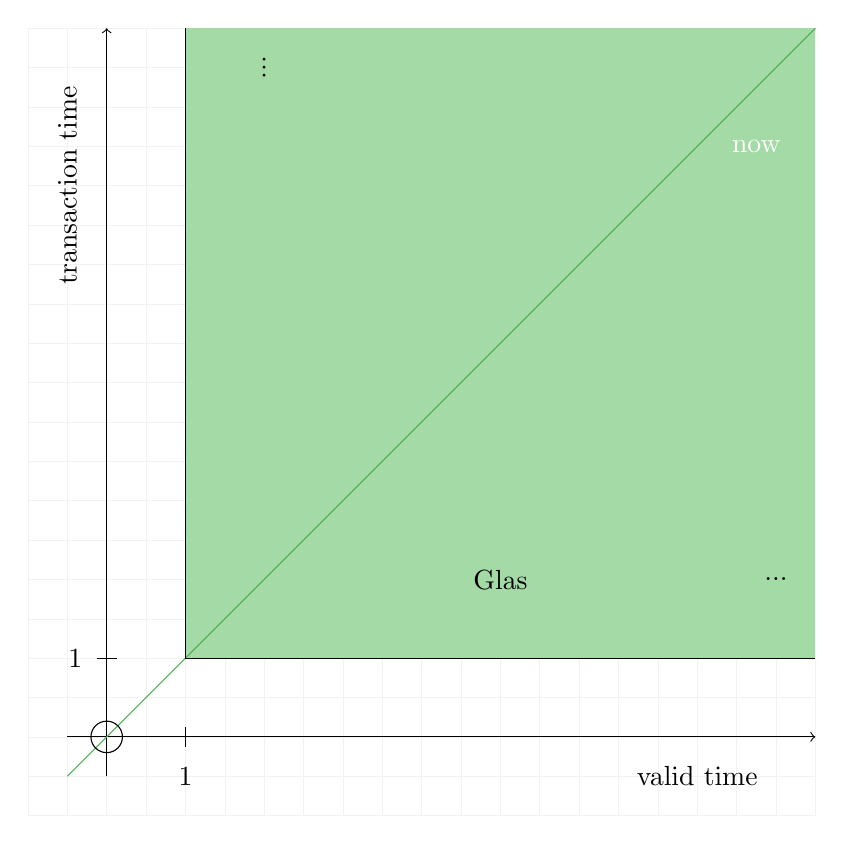
\begin{tikzpicture}
	\definecolor{brightgray}{rgb}{0.95, 0.95, 0.95}
	\definecolor{darkgreen}{RGB}{76, 175, 80}
	\definecolor{content1}{RGB}{163,218,165}
	\definecolor{content2}{RGB}{118,188,121}

	\draw[step=.5cm,brightgray,very thin] (-1,-1) grid (9,9);
	\draw[->](-0.5, 0) -- (9,0);
	\draw[->](0, -0.5) -- (0, 9);
	\fill[content1] (1,9) -- (1,1) -- (9,1) -- (9,9);

	\draw[darkgreen] (-0.5,-0.5) -- (9,9);
	\draw (0,0) circle [radius=0.2];
	\draw(-0.125, 1) -- (0.125, 1);
	\draw(1,-0.125) -- (1,0.125);
	\draw (1,9) -- (1,1) -- (9,1);

	\draw (-0.4, 1) node {1};
	\draw (1, -0.5) node {1};
	\draw (5,2) node {Glas};
	\draw[white](8.25,7.5) node {now};
	\draw(8.5, 2) node {...};
	\draw(2, 8.5) node [rotate=90] {...};
	\draw (7.5, -0.5) node {valid time};
	\draw (-0.5, 7) node [rotate=90] {transaction time};
\end{tikzpicture}
\caption{Time Diagram of a Current Insert}
\end{figure}

\subsection{Current Update}

\begin{itemize}
	\item 1: \texttt{currentInsert("Glass")}
	\item 3: \texttt{currentUpdate("Jar")}
\end{itemize}

\begin{table}[!ht]
\begin{tabular}{c  | c | c | c | c}
	vt start & vt end & tt start & tt end & value\\\hline
	1 & i & 1 & 3 & Glas \\\hline
	1& 3 & 3 & i & Glas \\\hline
	3 & i & 3 & i & Jar
\end{tabular}
\caption{Database after Current Update}
\end{table}

\begin{figure}[!ht]
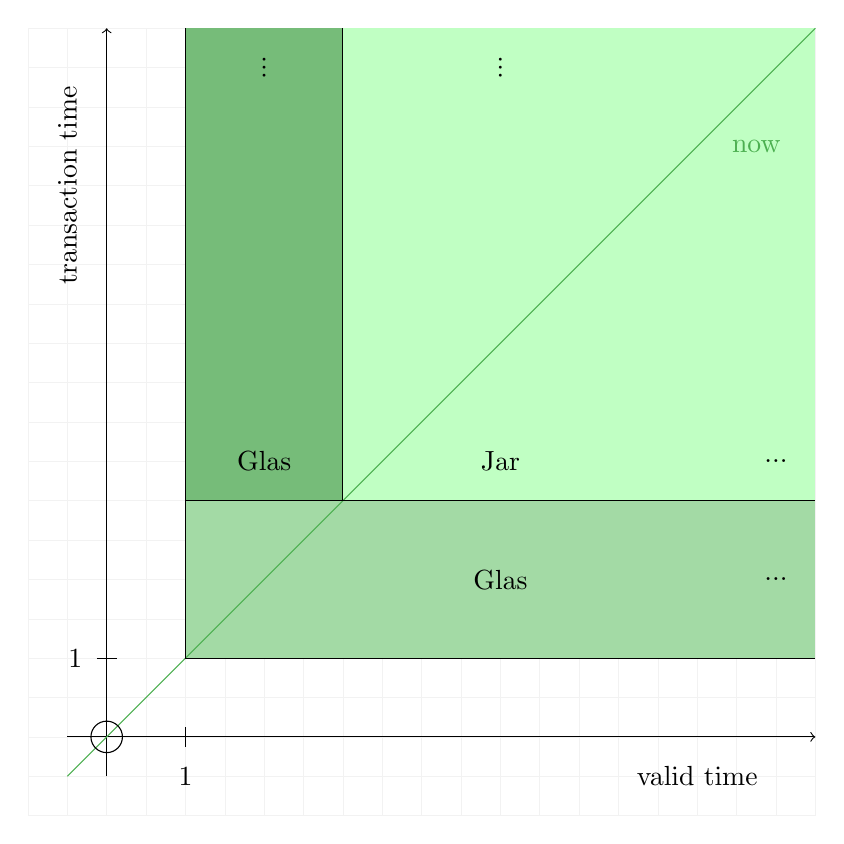
\begin{tikzpicture}
	\definecolor{brightgray}{rgb}{0.95, 0.95, 0.95}
	\definecolor{darkgreen}{RGB}{76, 175, 80}
	\definecolor{content1}{RGB}{163,218,165}
	\definecolor{content2}{RGB}{118,188,121}
	\definecolor{content3}{RGB}{192,255,195}

	\draw[step=.5cm,brightgray,very thin] (-1,-1) grid (9,9);
	\draw[->](-0.5, 0) -- (9,0);
	\draw[->](0, -0.5) -- (0, 9);
	\fill[content1] (1,3) -- (1,1) -- (9,1) -- (9,3);
	\fill[content2] (1,3) -- (3,3) -- (3,9) -- (1,9);
	\fill[content3] (3,9) -- (3,3) -- (9,3) -- (9,9);

	\draw[darkgreen] (-0.5,-0.5) -- (9,9);
	\draw (0,0) circle [radius=0.2];
	\draw(-0.125, 1) -- (0.125, 1);
	\draw(1,-0.125) -- (1,0.125);

	\draw (1,9) -- (1,1) -- (9,1);
	\draw (1,3) -- (3,3) -- (3,9);
	\draw (3,3) -- (9,3);

	\draw (-0.4, 1) node {1};
	\draw (1, -0.5) node {1};
	\draw (5,2) node {Glas};
	\draw (2,3.5) node {Glas};
	\draw (5, 3.5) node {Jar};
	\draw[darkgreen](8.25,7.5) node {now};
	\draw(8.5, 2) node {...};
	\draw(2, 8.5) node [rotate=90] {...};
	\draw(8.5, 3.5) node {...};
	\draw(5, 8.5) node [rotate=90] {...};
	\draw (7.5, -0.5) node {valid time};
	\draw (-0.5, 7) node [rotate=90] {transaction time};
\end{tikzpicture}
\caption{Time Diagram of a Current Update}
\end{figure}

\subsection{Current Delete}

\begin{itemize}
\item 1: \texttt{currentInsert("Glass")}
\item 3: \texttt{currentUpdate("Jar")}
\item 6: \texttt{currentDelete()}
\end{itemize}

\begin{table}[!ht]
\begin{tabular}{c  | c | c | c | c}
	vt start & vt end & tt start & tt end & value\\\hline
	1 & i & 1 & 3 & Glas \\\hline
	1& 3 & 3 & i & Glas \\\hline
	3 & i & 3 & 6 & Jar \\\hline
	3 & 6 & 6 & i & Jar
\end{tabular}
\caption{Database after Current Delete}
\end{table}

\begin{figure}[!ht]
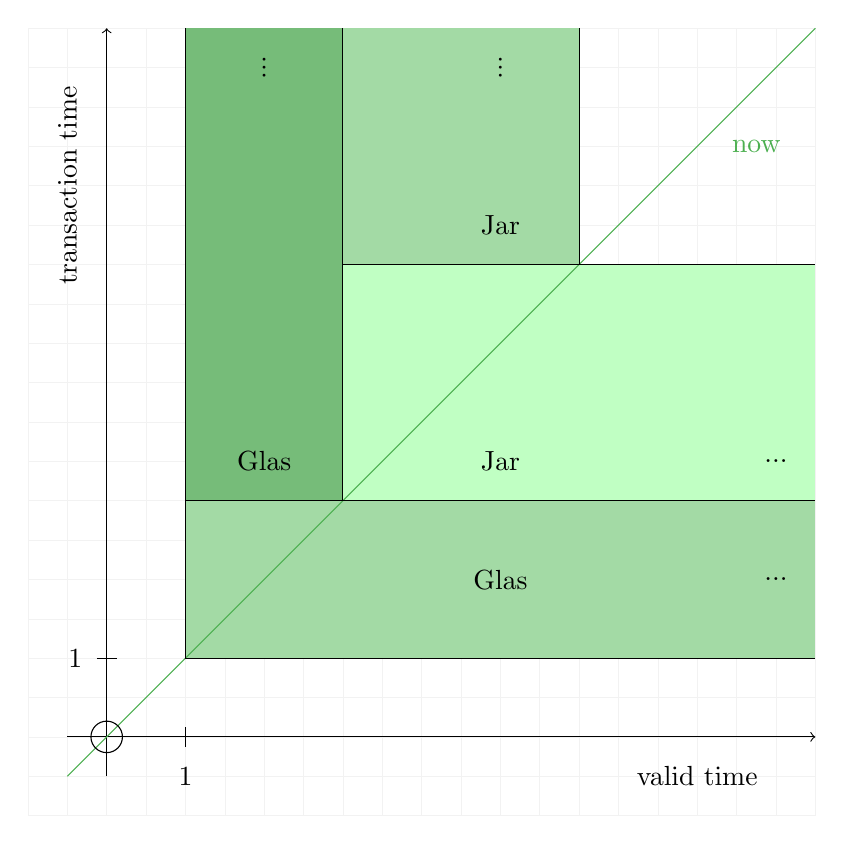
\begin{tikzpicture}
	\definecolor{brightgray}{rgb}{0.95, 0.95, 0.95}
	\definecolor{darkgreen}{RGB}{76, 175, 80}
	\definecolor{content1}{RGB}{163,218,165}
	\definecolor{content2}{RGB}{118,188,121}
	\definecolor{content3}{RGB}{192,255,195}

	\draw[step=.5cm,brightgray,very thin] (-1,-1) grid (9,9);
	\draw[->](-0.5, 0) -- (9,0);
	\draw[->](0, -0.5) -- (0, 9);
	\fill[content1] (1,3) -- (1,1) -- (9,1) -- (9,3);
	\fill[content2] (1,3) -- (3,3) -- (3,9) -- (1,9);
	\fill[content1] (3,9) -- (3,3) -- (6,3) -- (6,9);
	\fill[content3] (3,6) -- (3,3) -- (9,3) -- (9,6);

	\draw[darkgreen] (-0.5,-0.5) -- (9,9);
	\draw (0,0) circle [radius=0.2];
	\draw(-0.125, 1) -- (0.125, 1);
	\draw(1,-0.125) -- (1,0.125);

	\draw (1,9) -- (1,1) -- (9,1);
	\draw (1,3) -- (3,3) -- (3,9);
	\draw (3,3) -- (9,3);
	\draw (3,6) -- (6,6) -- (6,9);
	\draw (6,6) -- (9,6);

	\draw (-0.4, 1) node {1};
	\draw (1, -0.5) node {1};
	\draw[darkgreen](8.25,7.5) node {now};
	\draw (7.5, -0.5) node {valid time};
	\draw (-0.5, 7) node [rotate=90] {transaction time};

	\draw (5,2) node {Glas};
	\draw (2,3.5) node {Glas};
	\draw (5, 3.5) node {Jar};
	\draw (5,6.5) node {Jar};

	\draw(8.5, 2) node {...};
	\draw(2, 8.5) node [rotate=90] {...};
	\draw(8.5, 3.5) node {...};
	\draw(5, 8.5) node [rotate=90] {...};
\end{tikzpicture}
\caption{Time Diagram of a Current Delete}
\end{figure}

\subsection{Sequenced Delete}

\begin{itemize}
	\item 1: \texttt{currentInsert("Glass")}
	\item 3: \texttt{currentUpdate("Jar")}
	\item 6: \texttt{sequencedDeletion(1, i)}
\end{itemize}

\begin{table}[!ht]
\begin{tabular}{c  | c | c | c | c}
	vt start & vt end & tt start & tt end & value\\\hline
	1 & i & 1 & 3 & Glas \\\hline
	1& 3 & 3 & 6 & Glas \\\hline
	3 & i & 3 & 6 & Jar
\end{tabular}
\caption{Database after Sequenced Delete}
\end{table}

\begin{figure}[!ht]
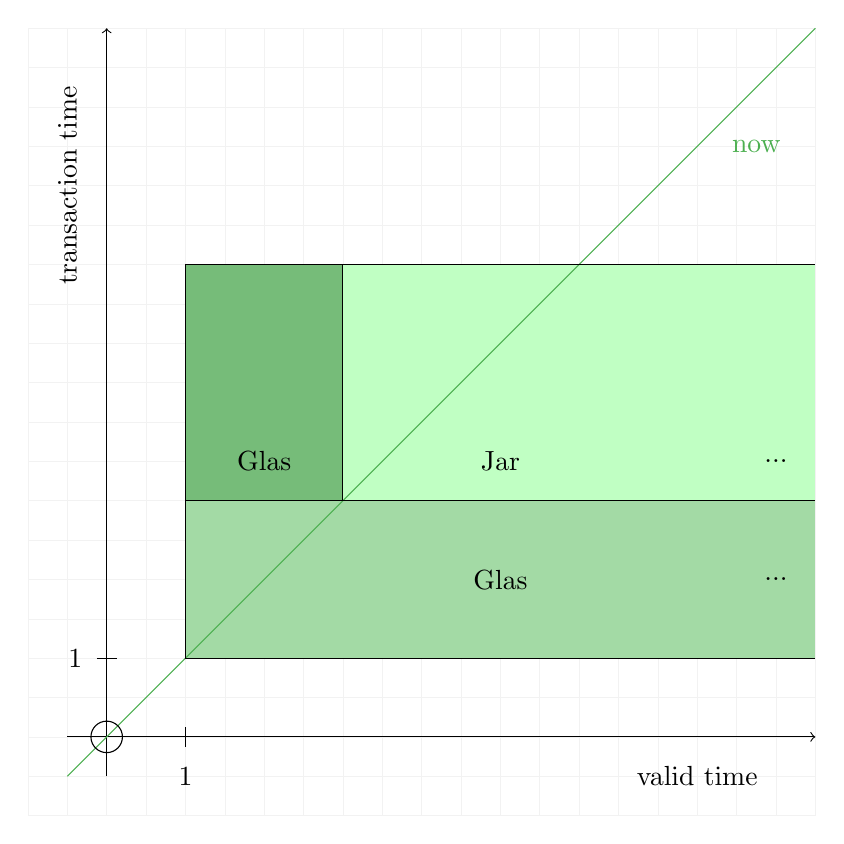
\begin{tikzpicture}
	\definecolor{brightgray}{rgb}{0.95, 0.95, 0.95}
	\definecolor{darkgreen}{RGB}{76, 175, 80}
	\definecolor{content1}{RGB}{163,218,165}
	\definecolor{content2}{RGB}{118,188,121}
	\definecolor{content3}{RGB}{192,255,195}

	\draw[step=.5cm,brightgray,very thin] (-1,-1) grid (9,9);
	\draw[->](-0.5, 0) -- (9,0);
	\draw[->](0, -0.5) -- (0, 9);
	\fill[content1] (1,3) -- (1,1) -- (9,1) -- (9,3);
	\fill[content2] (1,3) -- (3,3) -- (3,6) -- (1,6);
	\fill[content3] (3,6) -- (3,3) -- (9,3) -- (9,6);

	\draw[darkgreen] (-0.5,-0.5) -- (9,9);
	\draw (0,0) circle [radius=0.2];
	\draw(-0.125, 1) -- (0.125, 1);
	\draw(1,-0.125) -- (1,0.125);

	\draw (1,6) -- (1,1) -- (9,1);
	\draw (1,3) -- (3,3) -- (3,6) -- (1,6);
	\draw (3,3) -- (9,3);
	\draw (3,6) -- (9,6);

	\draw (-0.4, 1) node {1};
	\draw (1, -0.5) node {1};
	\draw[darkgreen](8.25,7.5) node {now};
	\draw (7.5, -0.5) node {valid time};
	\draw (-0.5, 7) node [rotate=90] {transaction time};

	\draw (5,2) node {Glas};
	\draw (2,3.5) node {Glas};
	\draw (5, 3.5) node {Jar};

	\draw(8.5, 2) node {...};
	\draw(8.5, 3.5) node {...};
\end{tikzpicture}
\caption{Time Diagram of a Sequenced Delete}
\end{figure}

\subsection{Sequenced Update}

\begin{itemize}
	\item 3: \texttt{sequencedUpdate(2 - 6, value2 := 0)}
\end{itemize}

\begin{table}[!ht]
\begin{tabular}{c  | c | c | c | c | c}
	vt start & vt end & tt start & tt end & value1 & value2\\\hline
	1 & 3 & 1 & 3 & a & 1 \\\hline
	3 & 5 & 1 & 3 & b & 2 \\\hline
	5 & i & 1 & 3 & c & 3 \\\hline
	1 & 2 & 3 & i & a & 1 \\\hline
	2 & 3 & 3 & i & a & 0 \\\hline
	3 & 5 & 3 & i & b & 0 \\\hline
	5 & 6 & 3 & i & c & 0 \\\hline
	6 & i & 3 & i & c & 3
\end{tabular}
\caption{Database after Sequenced Update}
\end{table}

\begin{figure}[!ht]
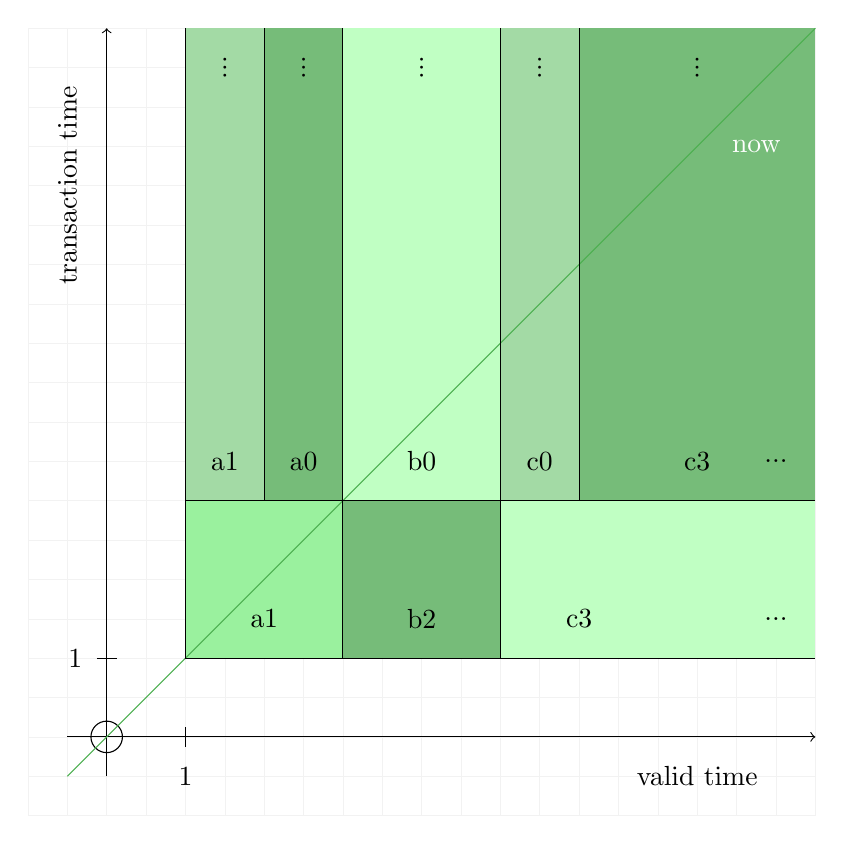
\begin{tikzpicture}
	\definecolor{brightgray}{rgb}{0.95, 0.95, 0.95}
	\definecolor{darkgreen}{RGB}{76, 175, 80}
	\definecolor{content1}{RGB}{163,218,165}
	\definecolor{content2}{RGB}{118,188,121}
	\definecolor{content3}{RGB}{192,255,195}
	\definecolor{content4}{RGB}{154,241,158}

	\draw[step=.5cm,brightgray,very thin] (-1,-1) grid (9,9);
	\draw[->](-0.5, 0) -- (9,0);
	\draw[->](0, -0.5) -- (0, 9);

	\draw (0,0) circle [radius=0.2];
	\draw(-0.125, 1) -- (0.125, 1);
	\draw(1,-0.125) -- (1,0.125);

	\fill [color=content1] (1,9) -- (1,3) -- (2,3) -- (2,9);
	\fill [color=content2] (2,9) -- (2,3) -- (3,3) -- (3,9);
	\fill [color=content4] (1,1) -- (1,3) -- (3,3) -- (3,1) -- (1,1);
	\fill [color=content2](3,1) -- (5,1) -- (5,3) -- (3,3) -- (3,1);
	\fill [color=content3] (5,1) -- (9,1) -- (9,3) -- (5,3);
	\fill [color=content3] (3,9) -- (3,3) -- (5,3) -- (5,9);
	\fill [color=content1] (5,9) -- (5,3) -- (6,3) -- (6,9);
	\fill [color=content2] (6,9) -- (6,3) -- (9,3) -- (9,9);

	\draw[darkgreen] (-0.5,-0.5) -- (9,9);

	\draw (1,9) -- (1,3) -- (2,3) -- (2,9);
	\draw (2,9) -- (2,3) -- (3,3) -- (3,9);
	\draw (3,9) -- (3,3) -- (5,3) -- (5,9);
	\draw (5,9) -- (5,3) -- (6,3) -- (6,9);
	\draw (6,9) -- (6,3) -- (9,3);
	\draw (1,1) -- (1,3) -- (3,3) -- (3,1) -- (1,1);
	\draw (3,1) -- (5,1) -- (5,3) -- (3,3) -- (3,1);
	\draw (5,1) -- (9,1);

	\draw (-0.4, 1) node {1};
	\draw (1, -0.5) node {1};
	\draw[white](8.25,7.5) node {now};
	\draw (7.5, -0.5) node {valid time};
	\draw (-0.5, 7) node [rotate=90] {transaction time};

	\draw (2,1.5) node {a1};
	\draw (4,1.5) node {b2};
	\draw (6,1.5) node {c3};
	\draw (1.5, 3.5) node {a1};
	\draw (2.5, 3.5) node {a0};
	\draw (4, 3.5) node {b0};
	\draw (5.5, 3.5) node {c0};
	\draw (7.5, 3.5) node {c3};

	\draw (1.5, 8.5) node [rotate=90] {...};
	\draw (2.5, 8.5) node [rotate=90] {...};
	\draw (4, 8.5) node [rotate=90] {...};
	\draw (5.5, 8.5) node [rotate=90] {...};
	\draw (7.5, 8.5) node [rotate=90] {...};
	\draw (8.5, 1.5) node {...};
	\draw (8.5, 3.5) node {...};
\end{tikzpicture}
\caption{Time Diagram of a Sequenced Update}
\end{figure}

\section{Error Recording}

To record an error of a failed write operation special care is needed to load
foreign keys of the entity whose write has failed. We consider an entity $E$
that is either inserted, updated or deleted. $E$ references a foreign entity $F$
via a field $f$.

\subsection{Insert}

If an Insert operation fails, the client-local transaction time $t$ of the table
of $F$ at the moment of failure will be used to load $F$. There are three steps
for resolution, the first two of them may fail, depending on the state of $F$:

\begin{enumerate}
    \item Try to load $F$ at valid time "now" and transaction time "infinity".
    \item Try to load $F$ at the latest valid time start before "now" and
            transaction time "infinity". This has to be done if $F$ has been
            current-deleted between recording the error and loading the error.
    \item Try to load $F$ at the latest valid time start before "now" and
            transaction time $t$. This has to be done if $F$ has been
            sequenced-deleted for the entire valid time between recording the
            error and loading the error.
\end{enumerate}

The procedure ensures that the most recent version of $F$ is used. So if $F$ has
been updated in the meantime this update will be considered when loading $F$ to
display the error details. Intuitively this means we first look at $F$ now as
best known, then we search to the left (valid time past) and potentially repeat
a search to the left at transaction time $t$. Note that each referenced foreign
entity table has to use its own client-local transaction time.

\subsection{Update}

This is analogous to insertion, as new foreign entities referenced may not be
valid at the time the update is performed.

In case the server replys that there is an update conflict we have to consider
loading the data of three different versions of $E$: The original version on the
server on which we based our own update, the local version representing our own
intent to change $E$ and the remote version which is the version now as best
known on the server. The remote version must exist or otherwise the server would
have replied with a "not found" error rather than a conflict.

\paragraph{Original}

The original version of $E$ has successfully been entered into the database.
Thus the client-local transaction time of $E$ serves as transaction time.

\paragraph{Remote}

The remote version of $E$ was valid when we tried to perform the update. Thus
the client-local execution time serves as transaction time when resolving $E$
and $F$. We accept minor clock desynchronisations which may lead to spurious
failures in high-write situations which we expect to not occur.

\paragraph{Local}

The local version of $E$ has never been valid. At execution time the referenced
$F$ could have already been sequenced-deleted, so execution time might be too
late. Any $F$ which could have been selected must have been valid at the
client-local transaction time of $F$ at execution time and thus it can serve as
transaction time.

\subsection{Delete}

Loading a foreign key of a deleted entity can use the same resolution process as
inserting. But instead of using the client-local transaction time of each
foreign entity separately the client-local transaction time of the entity to be
deleted $E$ can be used. As the entity has been successfully inserted before,
all foreign keys must have been valid at this point.

\chapter{}
\section{Data Model}

\begin{figure}[!ht]
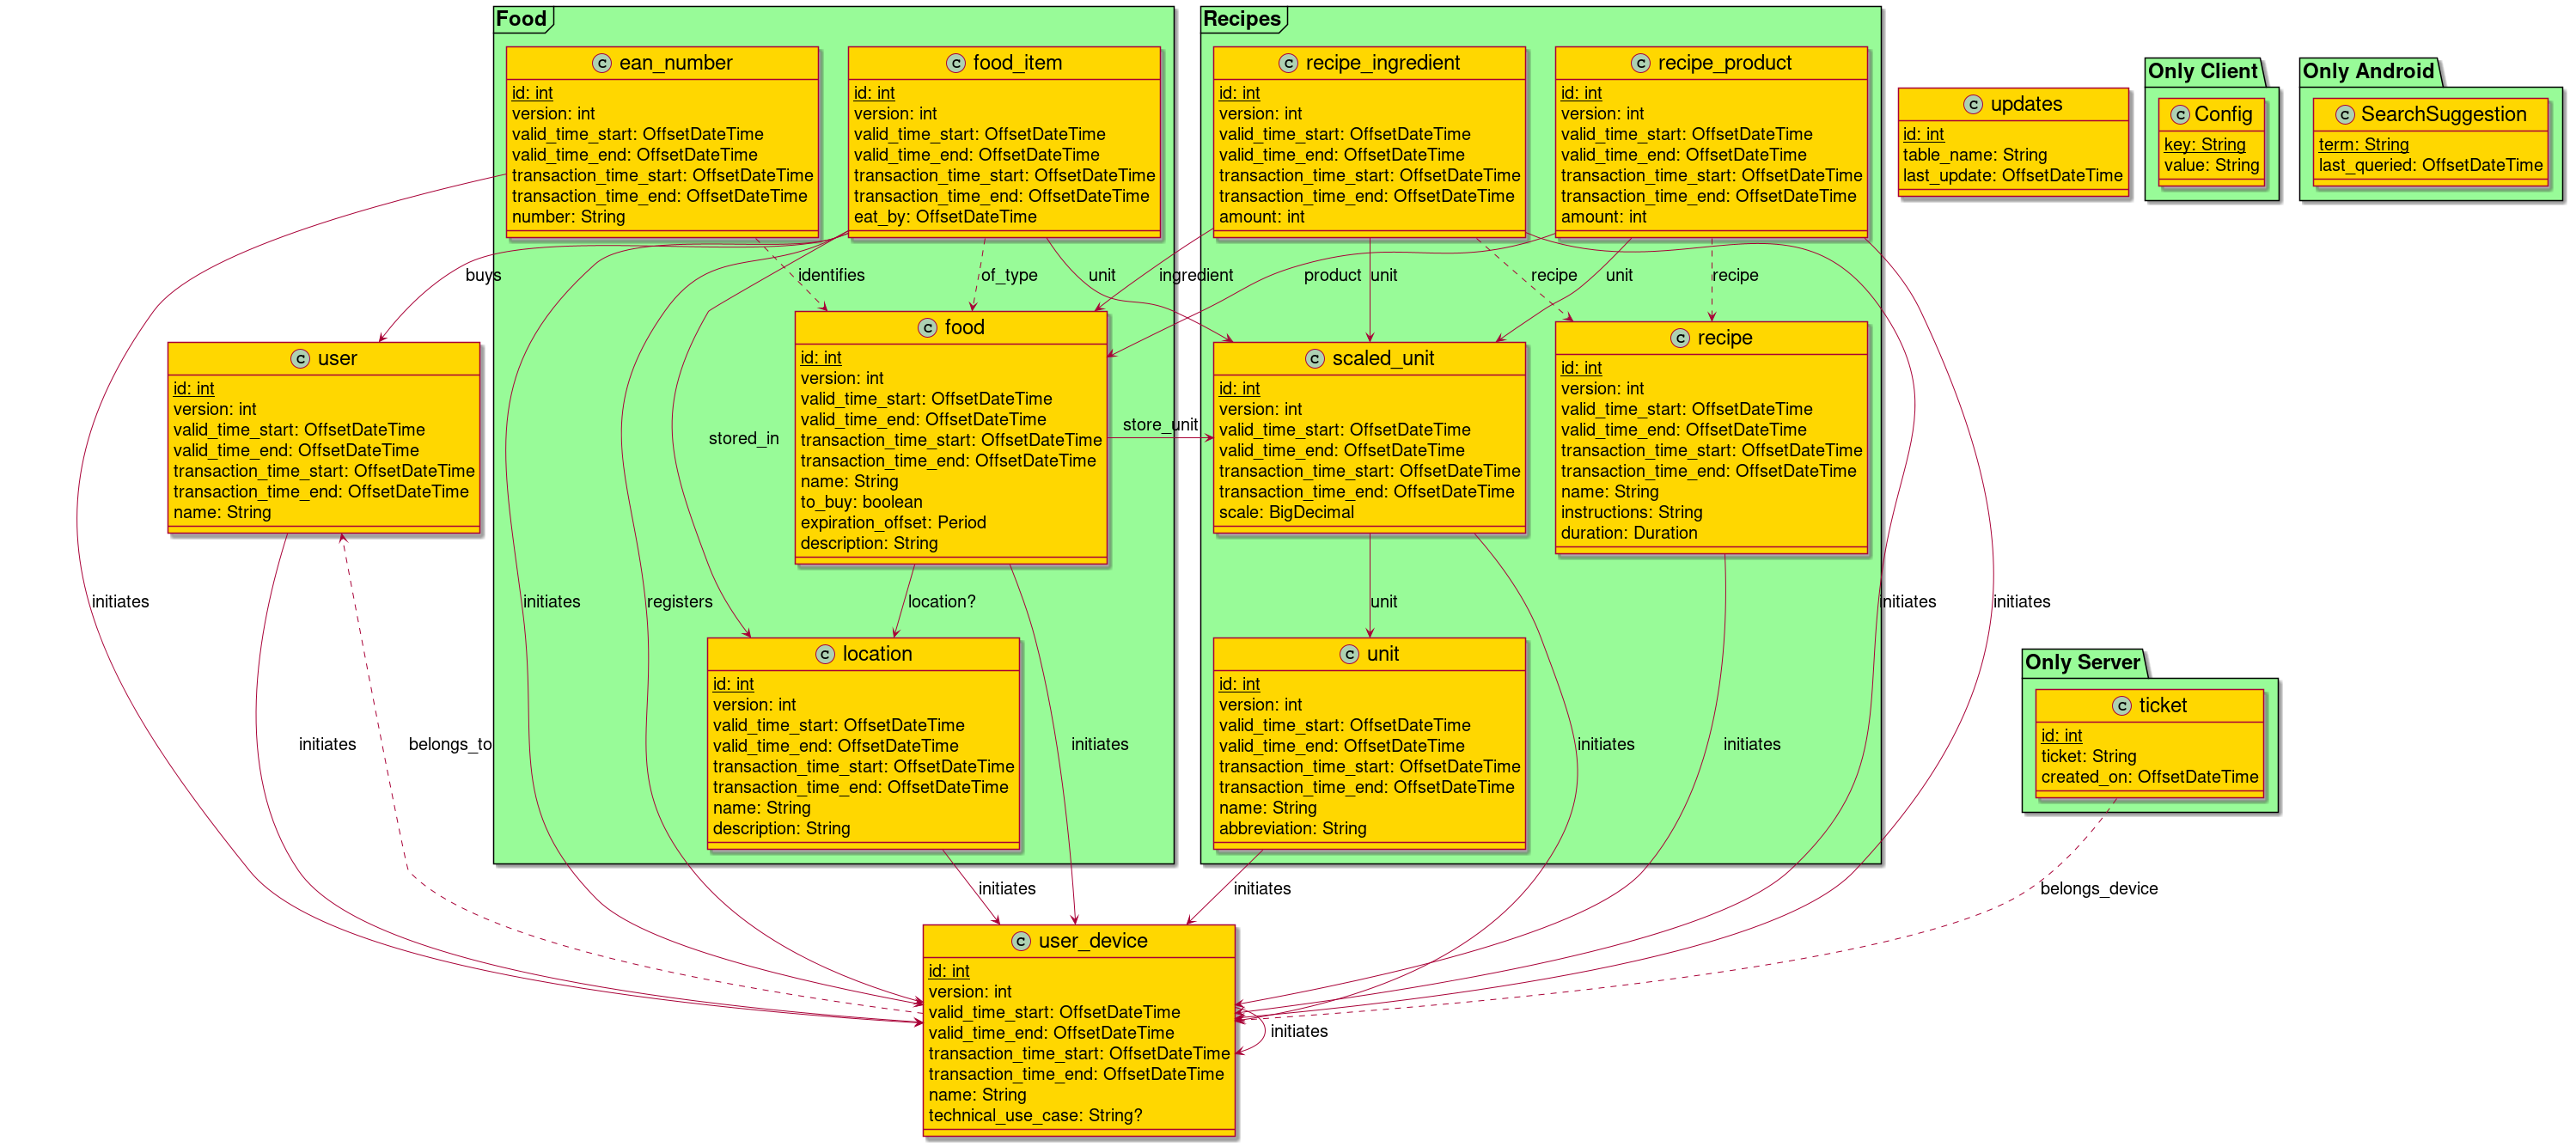
\includegraphics[width=\linewidth]{diagrams/data-model.png}
\caption{Data Model}
\end{figure}

\section{Architecture}

\subsection{Module Structure}

\begin{figure}[!ht]
\includegraphics[width=\linewidth]{diagrams/module-structure.png}
\caption{Module Structure}
\end{figure}

\subsection{Client}

Here interesting use cases for clients interacting with the server are
described.

\paragraph{Registering a New Data Item\\}

\begin{figure}[!ht]
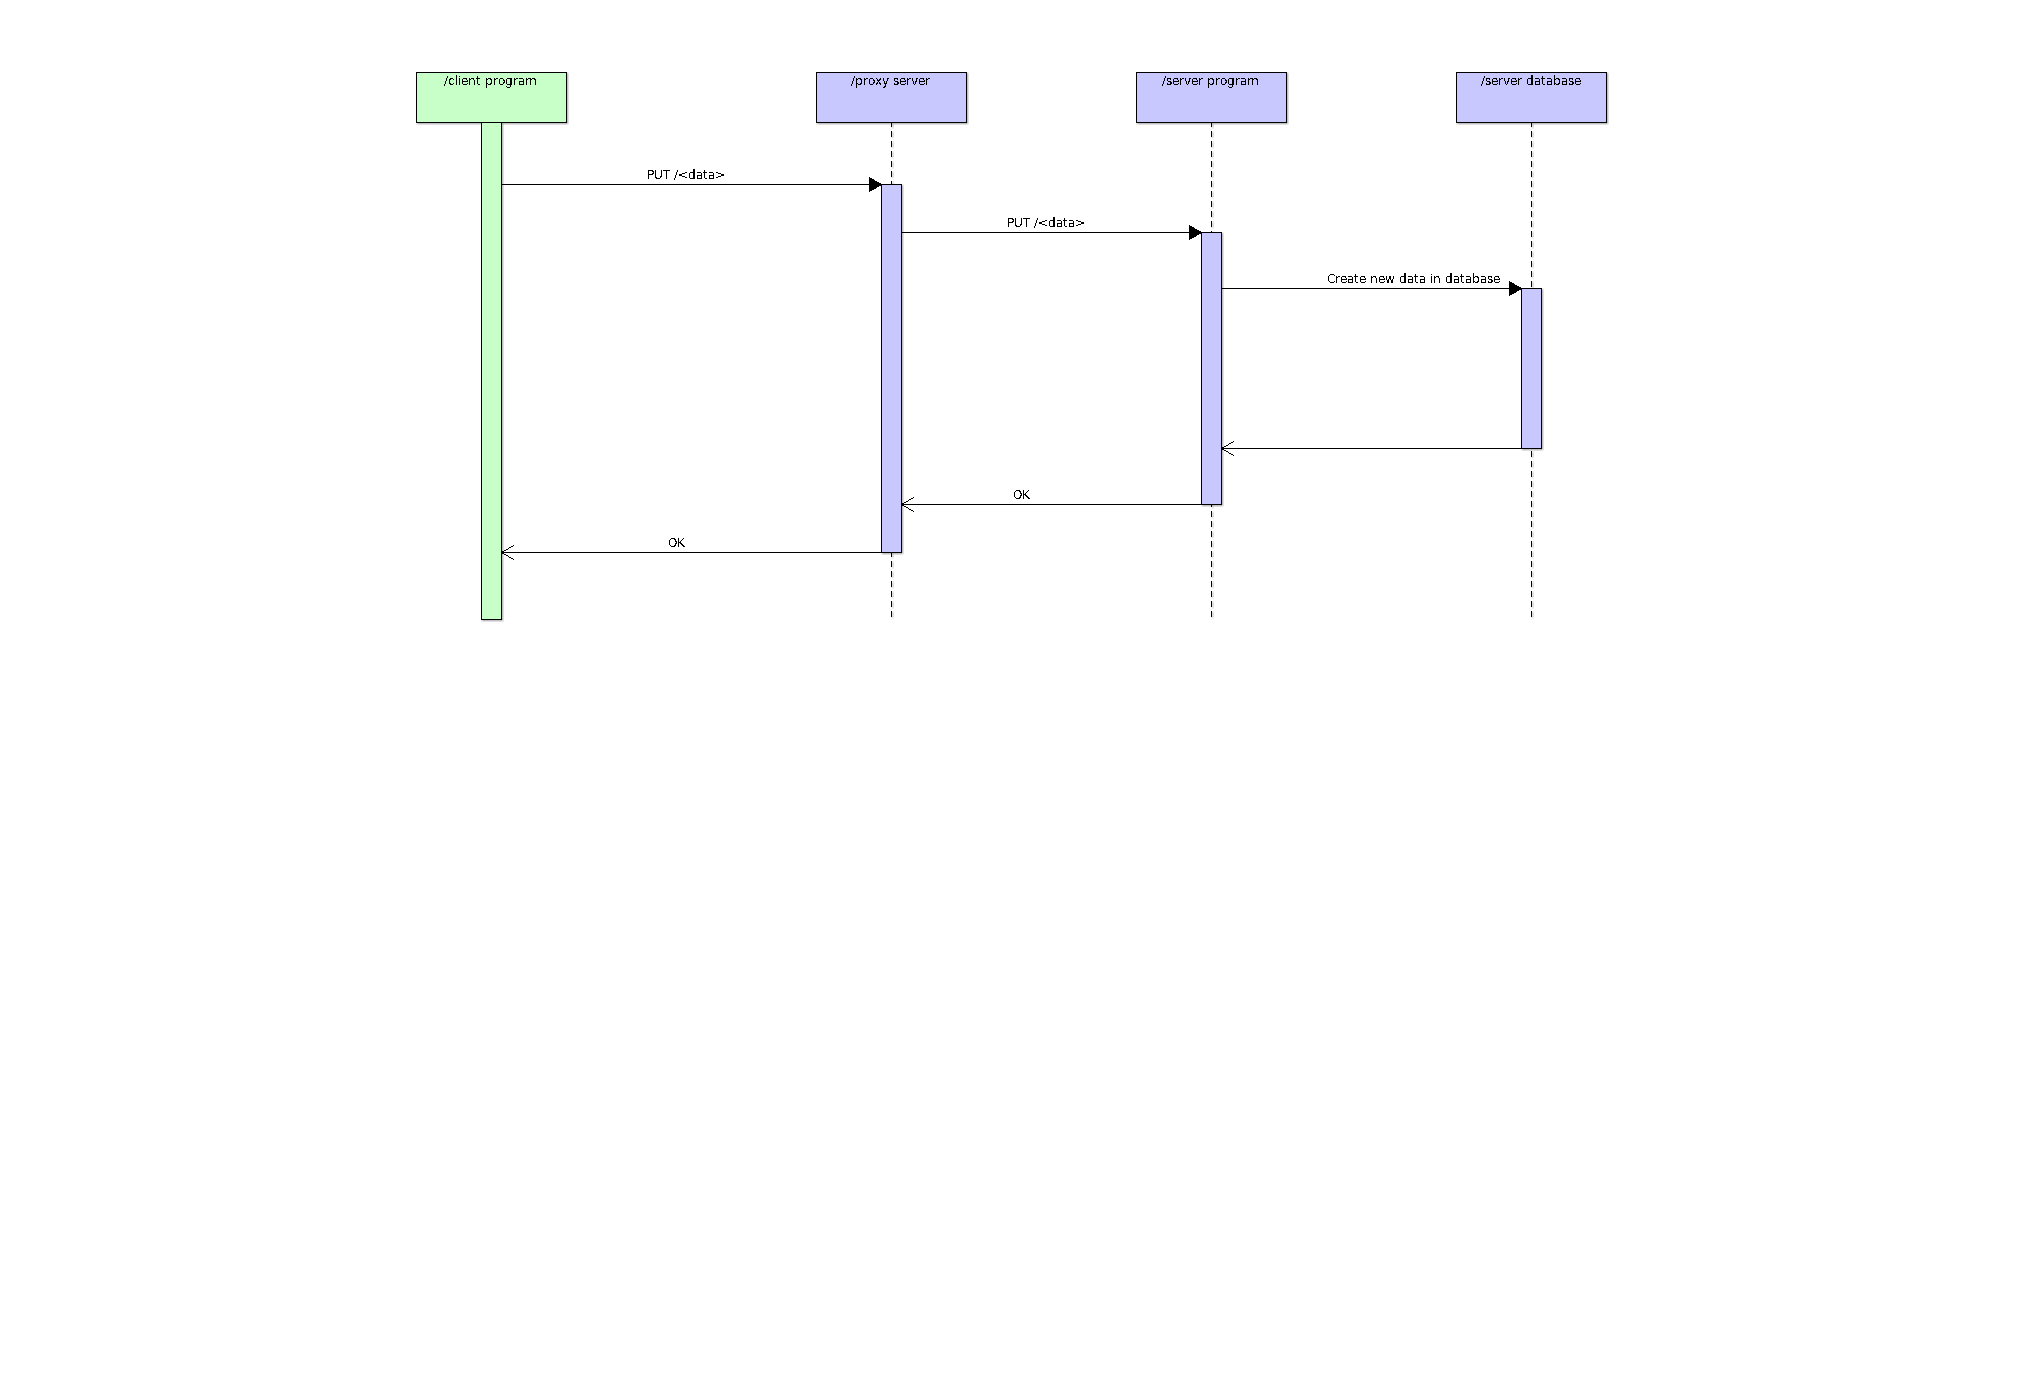
\includegraphics[width=\linewidth]{diagrams/put-data.png}
\caption{Write Operation}
\end{figure}

\paragraph{Refreshing the Client Database\\}

\begin{figure}[!ht]
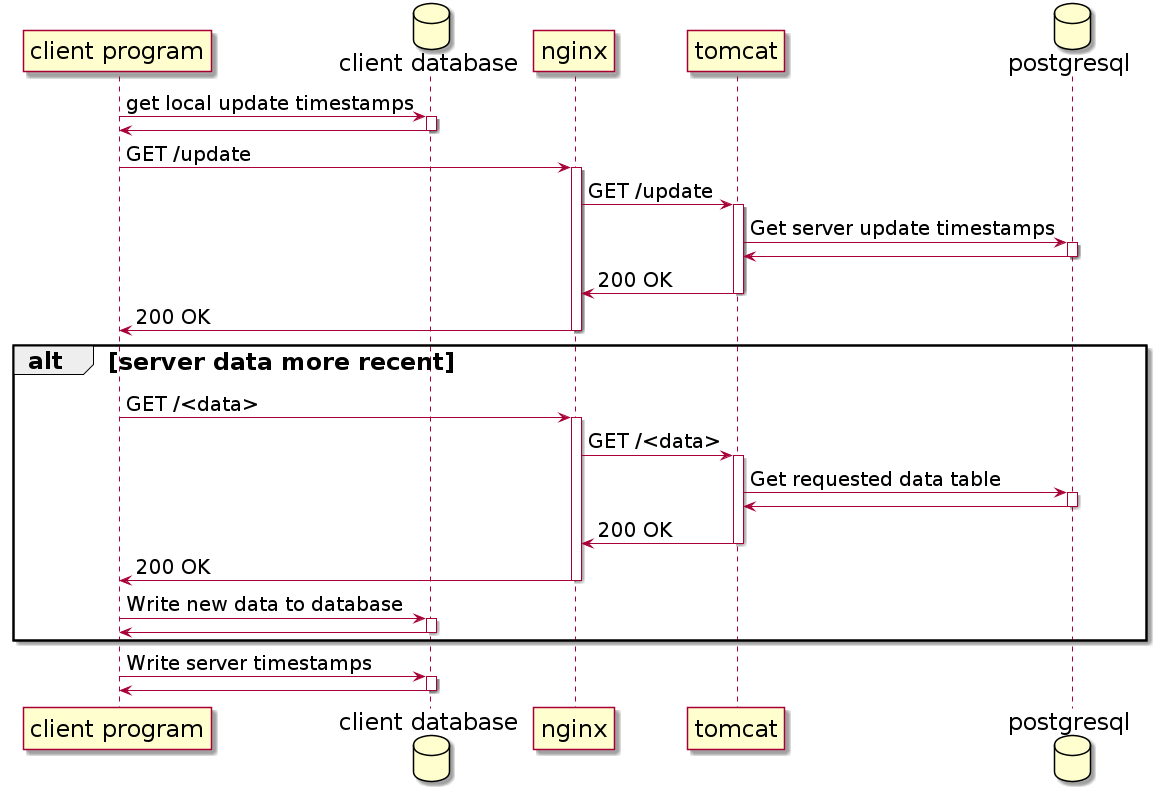
\includegraphics[width=\linewidth]{diagrams/refresh-data.png}
\caption{Refreshing Local Data}
\end{figure}

\paragraph{New Users' Registration}

New users are always added by giving a ticket from an existing user. The details
are outlined in the diagram.

\begin{figure}[!ht]
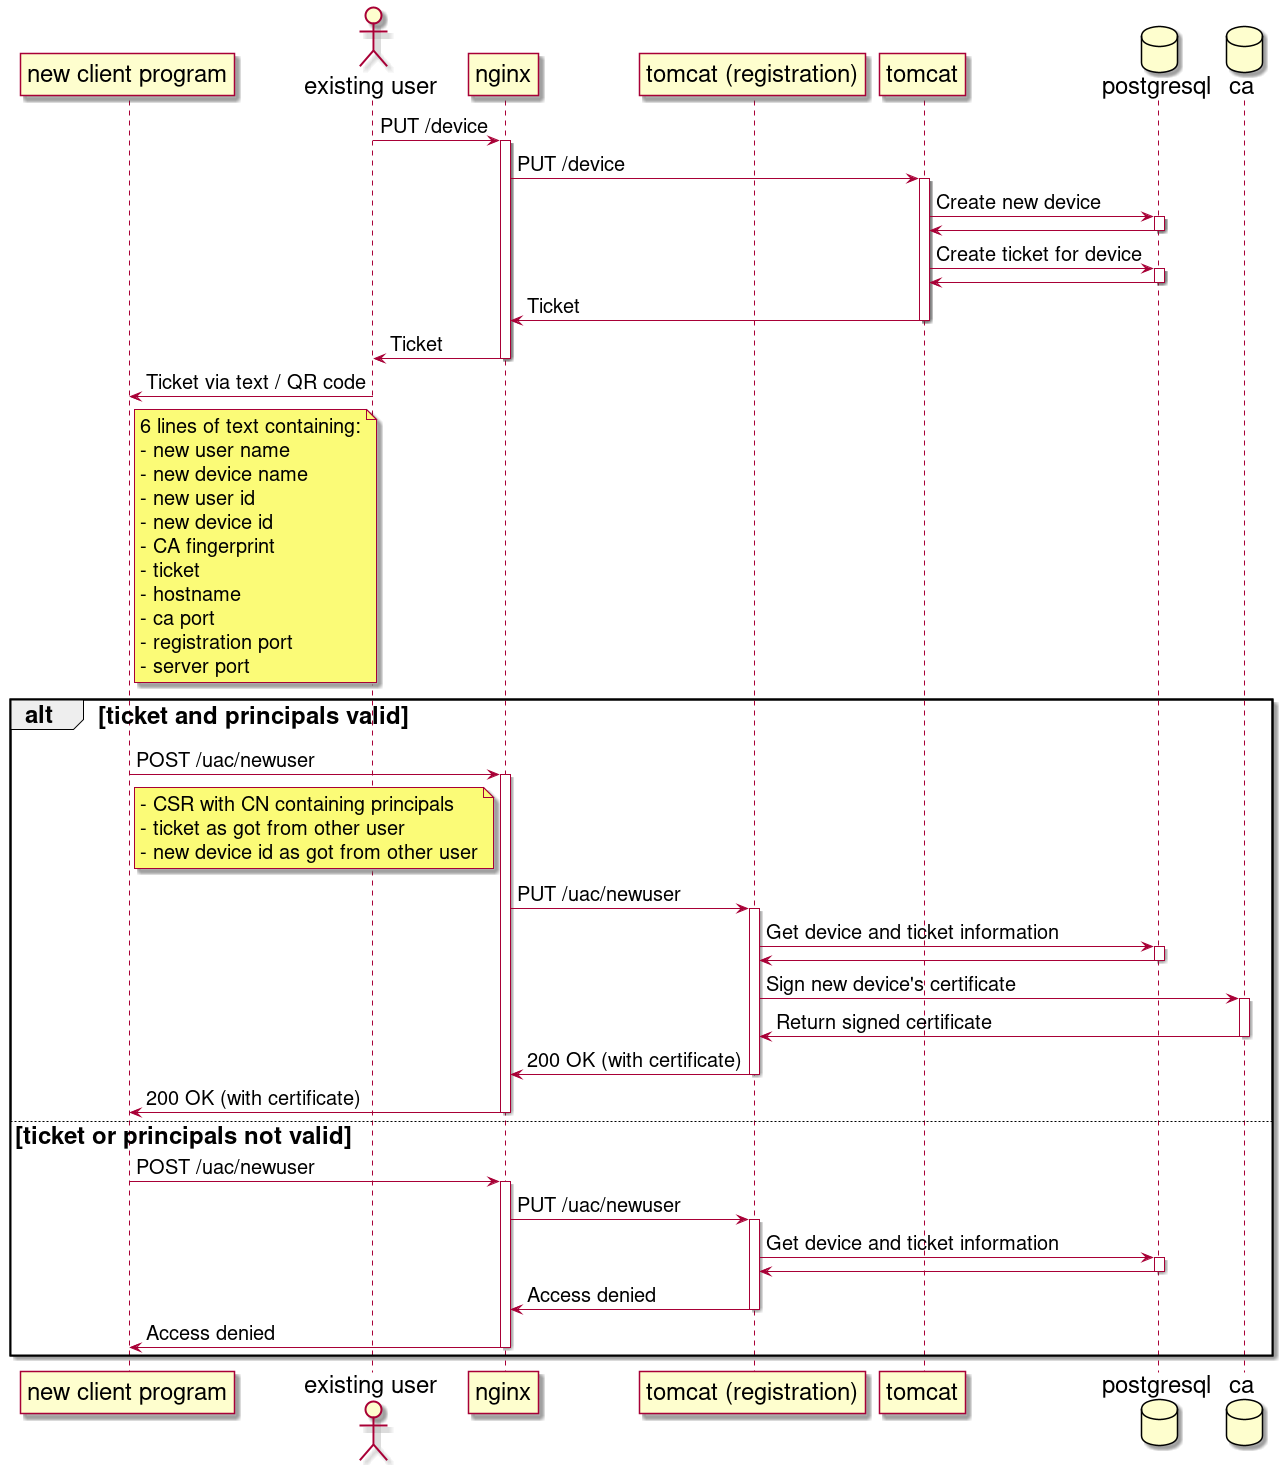
\includegraphics[width=\linewidth]{diagrams/device-registration.png}
\caption{Registering a new device}
\end{figure}

\paragraph{Principal Names}

In the CSR the user stores the principals of his device. The values are
formatted inside the Common Name attribute of the CSR. The pattern is
\texttt{username \$user\_id\$devicename\$ device\_id}. So for the default test
user this resolves to \texttt{Jack\$1\$Device\$1}. The principals are checked in
the sentry part of the server before the certificate is signed.

\paragraph{Client Verification}

Upon receiving a new device registration request, the sentry performs the
following checks in order:

\begin{itemize}
    \item Check if the ticket value presented by the client is found in the
            database
    \item Check the device id associated with the ticket from the database with
            the  device id from the CSR
    \item Check if the remaining principals of the device match the CSR
    \item Check if the ticket has expired
\end{itemize}

If all the checks succeed the sentry has the CSR signed by the CA and returns it
to the client.

\paragraph{QR Code Tickets}

For mobile clients it is more convenient to pass the ticket as QR code. To
generate this QR code the content of the ticket has to be entered text into the
QR code. The order of the values is the same as in the diagram description, i.e.

\begin{lstlisting}
Username
Device name
User ID
Device ID
CA Fingerprint
Ticket
hostname
ca port
registration port
server port
\end{lstlisting}

So for the default test user this resolves to

\begin{lstlisting}
Jack
Device
1
1
<some FPR>
0000
stocks.example
10910
10911
10912
\end{lstlisting}

\paragraph{Device Removal\\}

\begin{figure}[!ht]
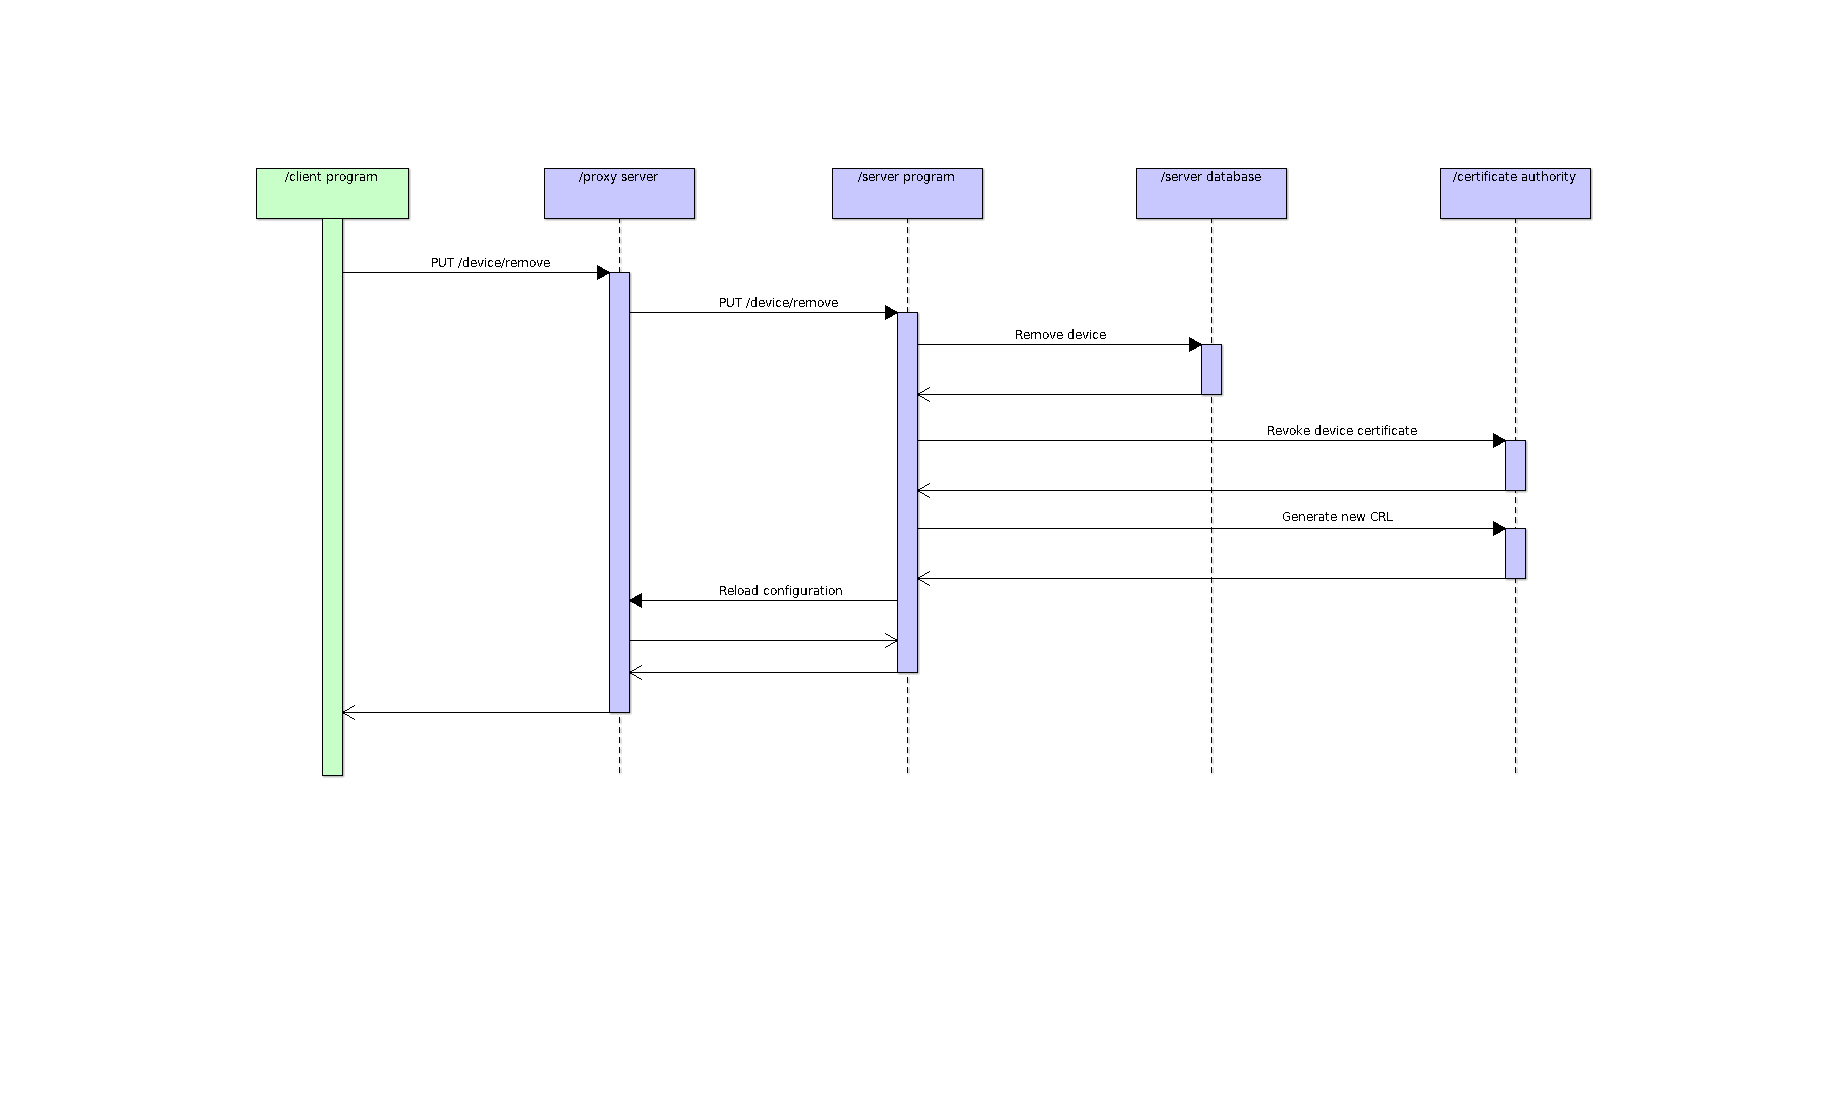
\includegraphics[width=\linewidth]{diagrams/remove-device.png}
\caption{Removing a Device}
\end{figure}

\section{Domain Language}

Registration: The request to get a new device's certificate from a CSR

Setup: The whole process of onboarding a new device. Includes Registration.

\section{REST API}

Get the server's API as \href{https://spec.openapis.org/oas/latest.html}{OpenAPI
specification} at \texttt{common/src/main/resources/api/openapi-spec.yaml}.

\backmatter

\bibliographystyle{unsrt}
\bibliography{refs}

\end{document}
